% Created 2017-04-29 六 17:40
\documentclass[11pt]{article}
\usepackage[utf8]{inputenc}
\usepackage[T1]{fontenc}
\usepackage{fixltx2e}
\usepackage{graphicx}
\usepackage{longtable}
\usepackage{float}
\usepackage{wrapfig}
\usepackage{rotating}
\usepackage[normalem]{ulem}
\usepackage{amsmath}
\usepackage{textcomp}
\usepackage{marvosym}
\usepackage{wasysym}
\usepackage{amssymb}
\usepackage{hyperref}
\tolerance=1000
\author{Qiu Wei, Wang Ruiji}
\date{\today}
\title{MPML REPORT}
\hypersetup{
  pdfkeywords={},
  pdfsubject={},
  pdfcreator={Emacs 24.5.1 (Org mode 8.2.10)}}
\begin{document}

\maketitle
\tableofcontents

\begin{abstract}
\ \ \ \ \ A method for machine learning to do classification in parallel is min-max modular. This method split problems with huge dataset into several smaller cases which can be finished in parallel. It can be designed as random or labeled min max algorithm which depends on the way separating the dataset. According to running time, F1 value and ROC curve, performance can be easily ranked comparing brute svm, using liblinear and min max modular in different ways.
\end{abstract}

\section{Introduction}
\label{sec-1}

\subsection{Binary classification}
\label{sec-1-1}
\ \ \ \ \ In machine learning, classification is the problem of identifying to which of a set of categories (sub-populations) a new observation belongs, on the basis of a training set of data containing observations (or instances) whose category membership is known. Classification is an example of pattern recognition.

Binary or binomial classification is the task of classifying the elements of a given set into two groups on the basis of a classification rule. Instancing a decision whether an item has or not some qualitative property, some specified characteristic.

\subsection{Problem explaination}
\label{sec-1-2}
\ \ \ \ \ This report will apply several methods to solve part of one classic problem called patent classification.

A patent classification is a system for examiners of patent offices or other people to code documents, such as published patent applications, according to the technical features of their content. Patent classifications make it possible to quickly find documents disclosing earlier disclosures identical or similar to the invention for which a patent is applied for.

The project dataset includes \emph{train.txt} (which contains 113128 samples) and \emph{test.txt} (which contains 37786 samples). Both of them are labeled and supposed to be separated into two specific parts. So it can be considered as a binary classification problem.

\subsection{Liblinear}
\label{sec-1-2}

\ \ \ \ \ Liblinear is a linear predictive models based on the 'LIBLINEAR' C/C++ Library. 'LIBLINEAR' is a simple library for solving large-scale regularized linear classification and regression. It currently supports L2-regularized classification as well as L1-regularized classification and L2-regularized support vector regression.

The main features of LiblineaR include multi-class classification (one-vs-the rest, and Crammer \& Singer method), cross validation for model selection, probability estimates (logistic regression only) or weights for unbalanced data. The estimation of the models is particularly fast as compared to other libraries.


\section{Min-max algorithm}
\label{sec-2}
\ \ \ \ \ The min-max algorithm partitions the positive set and negative set into
small parts, for example, the positive set is partitioned to n parts and
the negative set to m parts. Then build n*m svm models between these parts.
For each input, feed it to all the models, the result is:

$$ predict[i][j], i \in positive label, j \in negative label$$

Then the predicted class of this input is:

$$ max(min(predict[i][j], j \in negative label), i \in positive label)$$

This algorithm can improve the accuracy of classifier and avoid overfitting problem.
However, the penalty is that min-max algorithm need more time to train models and predict
the result. Another advantage is that it can be fully parallelized easily, and each single model
involves smaller data set. So it may even speed up the training phase in some cases.

The most important problem is which partition function to choose. Usually a partition function
should partition the data into proper number of parts, and have some structural reasons which
seperate similar data into the same set. In this experiment I choose two different partition function
to compare, the first one is partitioning randomly and the second one is partition by the first two
letter in the input's first label.

\section{Parallelization}
\label{sec-3}
\ \ \ \ \ Because of the GIL in python interpreter, multi-thread model do not help in this experiment.
The trainning phase and the testing phase is parallelized using multiprocessing module.
In trainning phase, each model is trained by a single process. In testing phase, batch predicting
is used and each process calculate the result of exactly one model.

The multi-process model is much safer than multi-thread model, in this case I just need to
join child process and get the result. However, the efficiency of multi-process is even
worse than serialized version in the beginning.

The first problem is fork() function will copy all the state of current program, which
copied the training data for multiple times. To deal with this problem, I write each part
of data set into a single file and read them in each child process so that I can release
the space of data set before fork().

Another problem is the big cost of frequent context switch. So I use Pool.map method of
multiprocessing module which runs exactly 4 processes in my 4-kernal machine. It also
reduces the space cost of the dead processes.

With these technich, the parallelized min-max algorithm is more than 2 times faster
compare with the serialized version.
The difference between multi-process and multi-thread is the big cost of message exchanging
which involves data copy in multi-process. For further optimization, using c to write the code
or call python in c code would be a good direction.

\section{Implementation}
\label{sec-4}
\ \ \ \ \ The python version is implemented with MPI,the source code is partitioned into several
parts via its functions. I will introduce the main structure of this project in the following.

\subsection{usage}
\label{sec-4-1}
\ \ \ \ \ To test a classifier, configure the algorithm in \emph{settings.py}. If min-max net algorithm
is used, specify the partition function in \emph{settings.py}, then run this command:
\begin{verbatim}
$ cd src/
$ python3 main.py
\end{verbatim}
\ \ \ \ \ In addition,if you want to run with the origin data, set PARSE\_DATA = True so
that the program will parse the origin data into .pickle files. The time of
parsing do not count in total time in timer class as you only need to parse the
data for just one time. Other advanced options can be found in the folloing part.

When all the algorithm have been tested, you can draw the ROC graph by \emph{drawroc.py}.
Run this command to draw ROC graph and calc AUC value:
\begin{verbatim}
$ python3 drawroc.py
\end{verbatim}

\subsection{structure}
\label{sec-4-2}
\ \ \ \ \ All the source code can be found in src/ folder. src/core/ stores the main part of
brute liblinear, serialized min-max and paralleled min-max algorithm. src/data/ stores
the training data, testing data and all the template .pickle files. src/models/ stores
all the svm models. src/tools/ stores many tool function for this project. src/timer/
contains timer class. src/utils/ contains util functions. src/settings.py contains
default settings. src/main.py is the main program. src/drawroc.py draw ROC graphs
via the result file in src/data/ folder.

\subsection{settings.py}
\label{sec-4-3}
\ \ \ \ \ The \emph{settings.py} file contains default settings of this project, containing default
algorithm, partition function in min-max algorithm,some constant and some folder/file name.
As there are no time to implement a parser, you must edit \emph{settings.py} to configure
the algorithm.

To start with, set the value of ALGORITHM
to specify which kind of algorithm you want and then set the value of PARTITION\_ALGORITHM to choose
partition function(labeled of randomed).

If you want to use post models for debugging, set MEMORIZE = True.
If you want to test the program in a smaller data set, set TRAIN\_DATA to your desired item numbers
greater than 0.
If you want to patition the items into a different number of sets in random labeled min-max net algorithm,
change the value of MAX\_CLASS to the max number of sets.

Other settings are seldom used and you can learn about their function by reading the source codes.

\subsection{utils and tools}
\label{sec-4-4}
\ \ \ \ \ The utils module comes from a repo in github, it mainly contains functional programming style
util functions such as partition, mapValue and mapv. A cd class is also contained to
ensure safe dictory switch.

src/tools stores the tools specificly designed for this project. \emph{partition.py} contains
partition functions used to partition data into different sets in min-max algorithm. \emph{dataIO.py}
implements the IO instruction with files. \emph{parseData.py} parses the origin data into a hash-map
in python, and dump it to a .pickle file. The main program will use the .pickle file directly
so this module will not be called in main program. \emph{tools.py} defines getModel, predictResult
,compareResult and metaNameFunc which will be used in all the three algorithms.

\subsection{drawroc.py}
\label{sec-4-5}
\ \ \ \ \ \emph{drawroc.py} use matplotlib.pyplot module to draw the ROC graph.
First it reads the result file of different algorithms, then call pyplot
to draw the ROC graph. Also the AUC value of the result is also calculated
and printed to the screen.
\subsection{timer}
\label{sec-4-6}
\ \ \ \ \ \emph{timer.py} uses time module to implement a multi-record timer. Different record
are stored in a hash-map and distinguished by its name. The start and end method
can start/end the timing a specific record. Also an add method is provided to
add a value to a record.
\subsection{core}
\label{sec-4-7}
\ \ \ \ The core module contains the main part of the program.
\emph{brute.py} use liblinear directly to solve the origin problem.
\emph{minmax.py} defines the abstraction of min-max algorithm and implements
the serialized version of this algorithm.
\emph{multiProc.py} implements the parallelized version of min-max algorithm.

All the algorithms contains a training phase and a testing phase, the time of
the two phases is rbecorded by the timer. The total time contains the time
cost of two phases and loading data.
\section{Trainning Result}
\label{sec-5}
The trainning result is as following:
\begin{center}
\begin{tabular}{rllrlrr}
\hline
No. & Algorithm & paralleled? & Time/s & Accuracy & F1 value & AUC value\\
\hline
1 & brute svm & $\backslash$ & 34.04 & 96.37167\% & 0.92404 & 0.98782\\
2 & random min-max & no & 305.47 & 96.26846\% & 0.92194 & $\backslash$\\
*2 & random min-max & no & 493.50 & 95.39777\% & 0.90679 & $\backslash$\\
3 & random min-max & yes & 140.08 & 96.26846\% & 0.92184 & 0.98307\\
4 & labeled min-max & no & 204.35 & 96.71042\% & 0.93101 & $\backslash$\\
*4 & labeled min-max & no & 2120.65 & 94.91081\% & 0.89781 & $\backslash$\\
5 & labeled min-max & yes & 204.35 & 96.69719\% & 0.93074 & 0.98567\\
\hline
\end{tabular}
\end{center}
\ \ \ \ \ The random min-max algorithm separate the input data into 5 parts randomly, which are 5*5 models.

(algorithm with * separate the positive data into 5 parts, negative parts into 15 parts, which are 5*15 models)

The labeled min-max separate the input data via the first two letters, which are 4*12 models.

(algorithm with * separate the positive data into 10 parts, negative parts into 32 parts, which are 10*32 models)

The total contains the time of load data, save model and other IO operations.
Parsing is finished before the program runs.

The ROC Graph is as following:


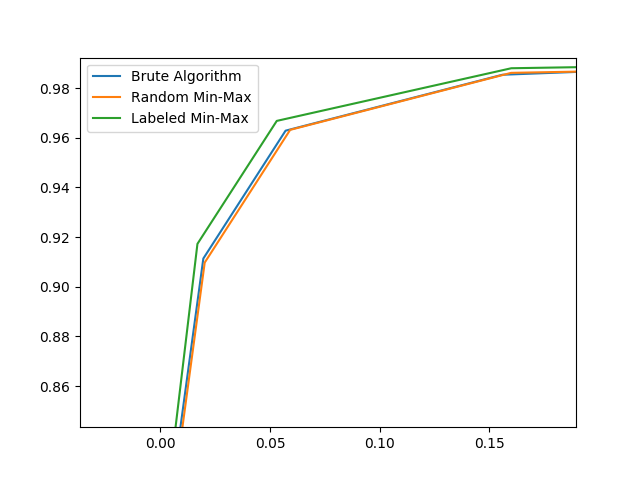
\includegraphics[width=.9\linewidth]{figure_1.png}



The time cost between serialized min-max and parallelized min-max is:

\begin{center}
\begin{tabular}{rlllll}
\hline
No. & Parallelized? & Algorithm & Trainning time & Testing time & Total time\\
\hline
1 & No & random & 103.98813 s & 200.19163 s & 305.47026 s\\
2 & Yes & random & 54.49303 s & 84.16756 s & 138.69087 s\\
3 & No & labeled & 115.96271 s & 371.83840 s & 489.00508 s\\
4 & Yes & labeled & 59.37346 s & 144.54046 s & 203.93383 s\\
\hline
\end{tabular}
\end{center}
Test environment:\\
Ubuntu, 4 kernel. Python version is 3.5.\\
MacOS(with *), 2 kernel. Python version is 2.7.\\
*Implement details please look up another pdf file.\\
\section{Analysis}

\subsection{F1 scores}
\label{sec-6-1}
\ \ \ \ \ The F1 score (also F-score or F-measure) is a measure of a test's accuracy. It considers both the precision p and the recall r of the test to compute the score: p is the number of correct positive results divided by the number of all positive results, and r is the number of correct positive results divided by the number of positive results that should have been returned. The F1 score can be interpreted as a weighted average of the precision and recall, where an F1 score reaches its best value at 1 and worst at 0.

The formulas are as follows:
\begin{equation}
F_1 = 2\times \frac{1}{\frac{1}{recall}+\frac{1}{precision}}
\end{equation}
\begin{equation}
recall = \frac{TP}{TP+FN}
\end{equation}
\begin{equation}
precision = \frac{TP}{TP+FP}
\end{equation}

\subsection{ROC curve}
\label{sec-6-2}
\ \ \ \ \ Receiver operating characteristic curve, or ROC curve, is a graphical plot that illustrates the performance of a binary classifier system as its discrimination threshold is varied.
The formulas are as follow:
\begin{equation}
TPR(True Positive Rate) = \frac{TP}{TP+FN}
\end{equation}
\begin{equation}
FPR(False Positive Rate) = \frac{FP}{FP+TN}
\end{equation}

\subsection{Comparison of the three algorithms}
\label{sec-6-3}
\ \ \ \ \ The best possible prediction method would yield a point in the upper left corner or coordinate (0,1) of the ROC space, representing 100\% sensitivity (no false negatives) and 100\% specificity (no false positives)

After plots of the three results above in the ROC space, we find that the result of Labeled Min-Max is clearly shows the best predictive power among all algorithms. The result of Random Min-Max and Brute Algorithm lie closely to each other, it can be seen that the accuracy of those two is almost the same. However, Brute algorithm shows slightly better result than Random Min-Max.
In this manner, we clearly say that the Labeled Min-Max algorithm gave the best result. Brute Algorithm performs slightly better than Random Min-Max.

In another hand, brute algorithm takes the least time in both training phase and testing phase. However, min-max algorithm can be fully-parallelized
easily, which makes it a better choice if we have more kernals. What is more, min-max algorithm can reduce the size of data in each training process,
which would be helpful when the time cost of training algorithm is sensitive with the size of data.

\subsection{Comparison between serial and paralleled}
\label{sec-6-4}
\ \ \ \ It's obviously that parallelized min-max algorithm takes less than half of the training time and testing time than relevant serial algorithm in 4-kernal machine. The main reason is that the multi-process model involves copy of data when exchanging messages between different process.

Each process must have a copy of data but share the data togother.In contrast, multi-thread model can share the memory between different threads,
which would be much more faster in this case.


\label{sec-5}
% Emacs 24.5.1 (Org mode 8.2.10)
\end{document}